\begin{frame}
\frametitle{SLAB Allocator}
\framesubtitle{Аллокация маленьких объектов фиксированного размера}

Теперь решаем еще более простую задачу - аллокацию "маленьких" объектов фиксированного размера:
\begin{itemize}
  \item мы умеем аллоцировать большие блоки - будем использовать их как пулы;
  \item аллоцируем блоки фиксированного размера из пула - тривиально;
  \item объекты одного размера уменьшают вероятность фрагментации;
  \item как на этом построить универсальный аллокатор (malloc/free)?
\end{itemize}

\end{frame}

\begin{frame}
\frametitle{SLAB Allocator}

Базовым понятием для SLAB аллокатора является (неожиданно) SLAB:
\begin{itemize}
  \item SLAB - это пулл объектов одинакового размера;
  \item аллокатор может имееть в распоряжении несколько SLAB-ов - при необходимости аллоцируются новые SLAB-ы;
  \item каждому объекту в SLAB-е соответствует дескриптор (по сути, нужен, чтобы связать объекты в список);
\end{itemize}
\end{frame}

\begin{frame}
\frametitle{SLAB Allocator}
\framesubtitle{Разделение на большие и маленькие объекты}

SLAB аллокатор делит объекты далее на большие и маленькие, и использует для них разную структуру SLAB-ов:
\begin{itemize}
  \item разделение нужно чтобы уменьшить потери памяти для больших объектов;
  \item нет четкой границы, что считать большим объектом, а что маленьким;
  \item обычно маленькими объектами считают объекты меньше $1/8$ размера PAGE (минимального размера пула).
\end{itemize}

\end{frame}

\begin{frame}
\frametitle{SLAB Allocator}
\framesubtitle{Организация SLAB-а маленьких объектов}

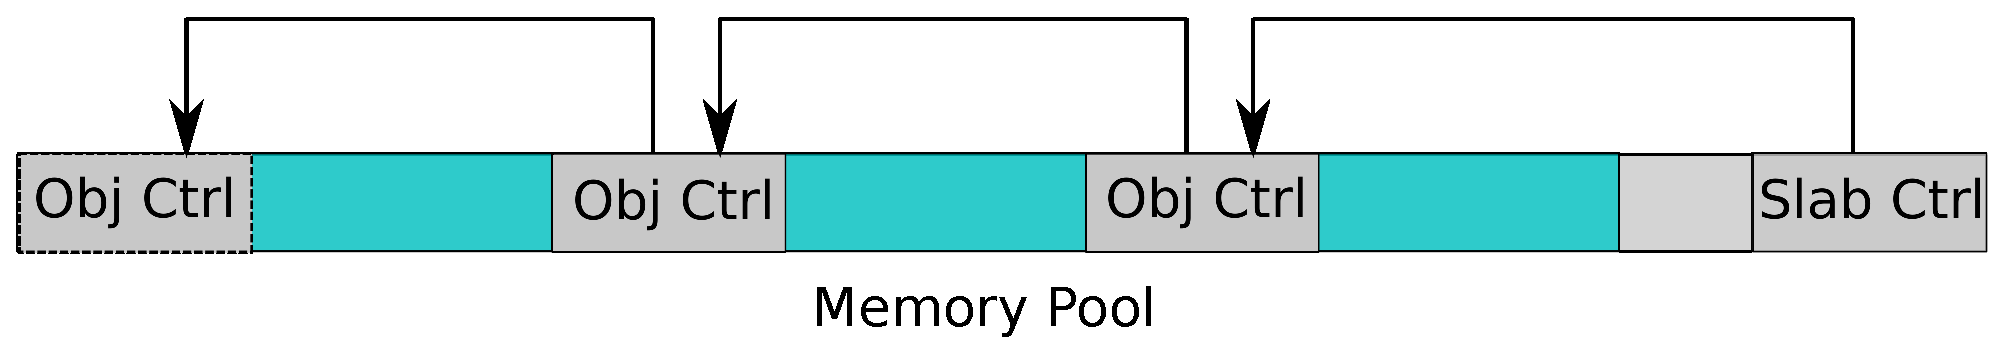
\includegraphics[width=.9\linewidth]{slab-small}

\end{frame}

\begin{frame}
\frametitle{SLAB Allocator}
\framesubtitle{Организация SLAB-а больших объектов объектов}

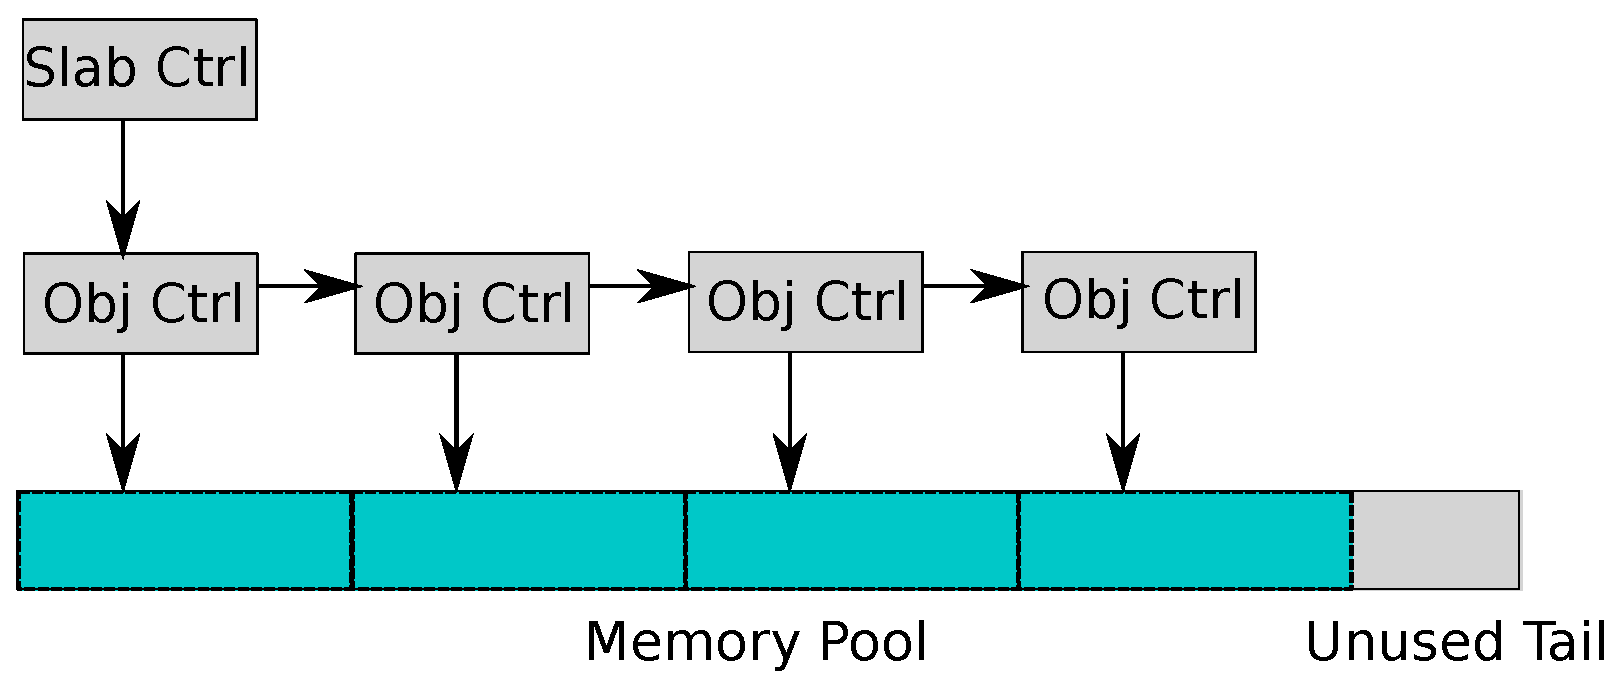
\includegraphics[width=.9\linewidth]{slab-large}

\end{frame}

\begin{frame}
\frametitle{SLAB Allocator}
\framesubtitle{Детали реализации}

\begin{itemize}
  \item Для SLAB-ов больших объектов управляющие структуры нужно аллоцировать отдельно - используя SLAB-ы маленьких объектов.
  \item При освобождении объекта нам нужно найти SLAB из которого он аллоцирован, это можно делать используя словарь (dict, map) или (гораздо проще) используя дескриптор PAGE.
  \item Для SLAB-ов больших объектов ObjCtrl необходим только когда объект свободен, когда объект объект был аллоцирован ObjCtrl больше не нужен.
  \item Аллокатор должен поддерживать набор SLAB-ов, т. е. возможно ему придется сосздавать новые SLAB-ы, если старые SLAB-ы заняты.
\end{itemize}
\end{frame}

\begin{frame}
\frametitle{SLAB Allocator}
\framesubtitle{malloc/free}

Используя Buddy Allocator и Slab Allocator можно создать аллокатор общего назначения (malloc/free):
\begin{itemize}
  \item Buddy Allocator - для аллокации пулов памяти для SLAB-ов и для аллокации памяти для больших объектов;
  \item набор предварительно созданных SLAB Allocator-ов с разными размерами объектов - для аллокации маленьких объектов;
\end{itemize}
\end{frame}

\begin{frame}
\frametitle{SLAB Allocator}
\framesubtitle{Объекты одного типа}

Мы можем создавать SLAB Allocator-ы под специфичные нужды и не использовать аллокатор общего назначения:
\begin{itemize}
  \item можно повысить надежность - уменьшив вероятность, что кто-то, по ошибке, испортит нашу память, или, наоборот, что мы испортим чужую;
  \item меньше конкуренция за ресурсы - аллокатором общего назначения пользуются все, а специальным аллокатором только мы;
  \item можно сэкономить на инициализации (далее подробнее);
\end{itemize}
\end{frame}

\begin{frame}
\frametitle{SLAB Allocator}
\framesubtitle{Объекты одного типа}

Многие поля объекта естественным образом оказываются в "иницализированном" состоянии при освобождении объекта:

\begin{itemize}
  \item если объект хранит mutex или spinlock (или какой-то другой примитив синхронизации), то перед освобождением он должен быть отпущен;
  \item если объект хранит счетчик ссылок, то перед освобождением он, зачастую, равен нулю;
  \item если объект хранит список или корень дерева, то перед освобождением они, зачастую, будут пустыми;
\end{itemize}

Такие поля достаточно инициализировать один раз -- экономия на инициализации.

\end{frame}

\begin{frame}
\frametitle{SLAB Allocator}
\framesubtitle{Cache Coloring}

Иногда, при использовании SLAB Allocator-а для достаточно больших объектов, в пуле памяти могут быть неиспользуемые "хвосты" - размер пула не делится нацело на размер объекта.

Этим неиспользуемым хвостам можно найти полезное применение - Cache Coloring.

\end{frame}

\begin{frame}
\frametitle{SLAB Allocator}
\framesubtitle{Cache Coloring}

\begin{columns}[T]

  \begin{column}{.3\textwidth}
    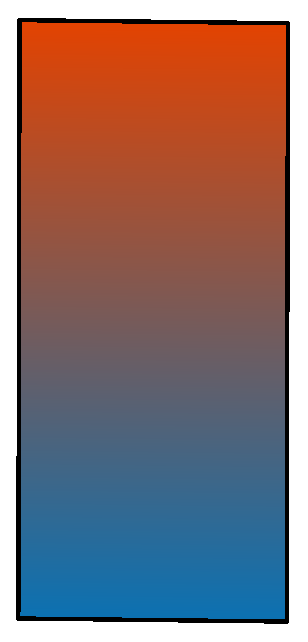
\includegraphics[width=.8\linewidth]{obj-hotmap}
  \end{column}

  \begin{column}{.7\textwidth}
    \begin{itemize}
      \item "горячие" поля, обычно, в начале:
        \begin{itemize}
          \item указатели (следующий/предыдущий, левый/правый)
          \item ключи для поиска (обычно короткие)
          \item флаги и примитивы синхронизации
        \end{itemize}
      \item "холодные" поля, обычно, в конце:
        \begin{itemize}
          \item значения, которые мы ищем (могут быть большими)
        \end{itemize}
    \end{itemize}
  \end{column}

\end{columns}

\end{frame}

\begin{frame}
\frametitle{SLAB Allocator}
\framesubtitle{Cache Coloring}

\begin{columns}[T]

  \begin{column}{.3\textwidth}
    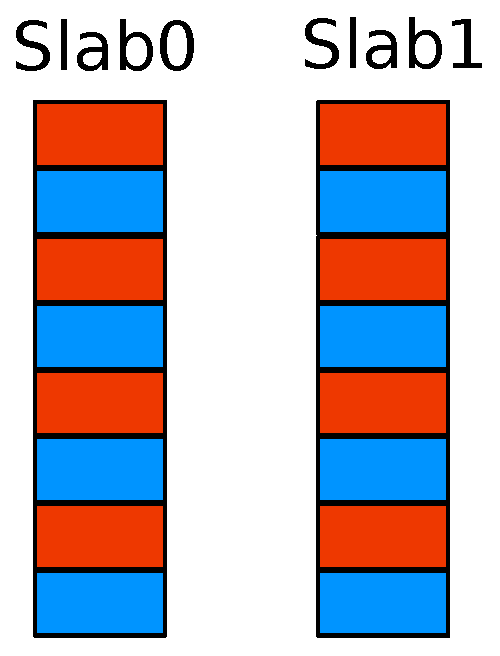
\includegraphics[width=\linewidth]{slab-color0}
  \end{column}

  \begin{column}{.7\textwidth}
    \begin{itemize}
      \item "горячие" поля обектов в Slab0 конкурируют с "горячими" полями объектов в Slab1 за место в процессорном кеше
      \item "холодные" поля конкурируют с "холодными" полями
      \item "холодные" поля используются редко - растрата кеша, лучше поделить его между "горячими" полями
    \end{itemize}
  \end{column}

\end{columns}

\end{frame}

\begin{frame}
\frametitle{SLAB Allocator}
\framesubtitle{Cache Coloring}

\begin{columns}[T]

  \begin{column}{.3\textwidth}
    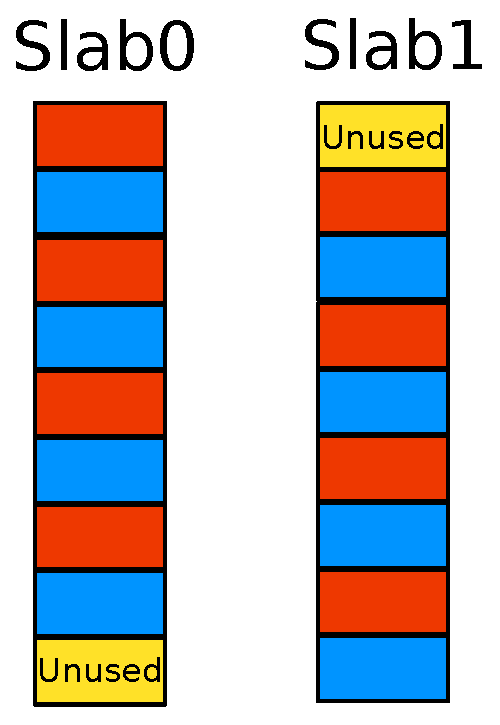
\includegraphics[width=\linewidth]{slab-color1}
  \end{column}

  \begin{column}{.7\textwidth}
    \begin{itemize}
      \item "горячие" поля обектов в Slab0 и Slab1 занимают весь кеш
      \item "холодные" поля поднимаются в кеш, только когда они нужны
    \end{itemize}
  \end{column}

\end{columns}

\end{frame}

